\chapter{Relevant Background}
\section{Data set}

In the context of Computer Science, very often our goal is to develop machines that can assist or automate the process of solving real-world problems. Firstly, however, we must find ways to express these problems numerically. This is where ``data sets" come in.

Although the recurrent usage of the term ``data set" in scientific work, there is not a clear definition established. It is possible, however, to observe the regular presence of four related features: grouping, content, relatedness and purpose \cite{ren2010}.
For the scope of this work, the term data set is invariably associated with the idea of a collection of samples. Each sample is a sequence of features, where the {\em i-th} feature of all instances belong to a same set of symbols $f_i$.

Succinctly, let $S$ be a set of samples and $F \coloneqq  \{f_i \mid f_i \textnormal{ is a set of symbols}\}$.
Then, the dataset $\vect X$ is defined as:
$$\vect X \coloneqq [x_{ij}] \mid x_{ij} \in f_j, \forall i \in [1, |S|], \forall j \in [1, |F|]$$

\subsubsection{Example of a canonical data set} \label{irisdataset}

The table bellow illustrates an example of data set, where each row represents a \textbf{sample}, and each column a \textbf{feature}.

\begin{table}[H]
	\begin{tabular}{ c || *{5}{c|}}
		& \textbf{Sepal length} & \textbf{Sepal width} & \textbf{Petal length} & \textbf{Petal width} & \textbf{Species} \\
		\hline
		1 & 5.1	& 3.5 & 1.4 & 0.2 & I. setosa \\
		2 & 4.9 & 3.0 & 1.4 & 0.2 & I. setosa \\
		3 & 4.7 & 3.2 & 1.3 & 0.2 & I. setosa \\
		… & … & … & … & … & … \\
	\end{tabular}
	\caption{The first three samples of the Iris flower data set \cite{lichman2013}.}
\end{table}

Iris flower is an example of data set broadly used in machine learning demonstrations, being usually interpreted as a classification problem where the feature {\em Species} will be learned from its adjacent features. In that scenario, {\em Species} is denominated \textbf{target feature}.

\subsection{Data set as a collection of vectors in the $\mathbb{R}^n$}

A data set can have each one of its nominal features enumerated, i.e., mapped to an element of $\mathbb{N}$. Such set could then be expressed as a collections of vectors in the $\mathbb{R}^n$. Consider the data set bellow:

\begin{table}[H]
	\begin{tabular}{ c | *{11}{|c}| }
		& \textbf{Age}
		& \textbf{Gen.}
		& \textbf{TB}
		& \textbf{DB}
		& \textbf{Alk.}
		& \textbf{Sgpt}
		& \textbf{Sgot}
		& \textbf{TP}
		& \textbf{ALB}
		& \textbf{A/G}
		& \textbf{S} \\
		\hline
		1 & 65 & Female & 0.7 & 0.1 & 187 & 16 & 18 & 6.8 & 3.3 & 0.9 & 1 \\
		2 & 62 & Male & 10.9 & 5.5 & 699 & 64 & 100 & 7.5 & 3.2 & 0.74 & 1 \\
		3 & 62 & Male & 7.3 & 4.1 & 490 & 60 & 68 & 7 & 3.3 & 0.89 & 1\\
		… & … & … & … & … & … & … & … & … & … & … & … \\
	\end{tabular}

	\caption{The first three samples of the Indian Liver Patient Dataset (ILPD) \cite{lichman2013}.}
\end{table}

Composed by 583 samples and 11 features, the data set ILPD has a nominal feature $Gender \coloneqq \{Male, Female\}$. {\em Gender} can, of course, be mapped on $\{0, 1\}$. ILPD can finally be expressed by the figure bellow:

\begin{figure}[H]
	\centering
	\captionsetup{justification=centering}

	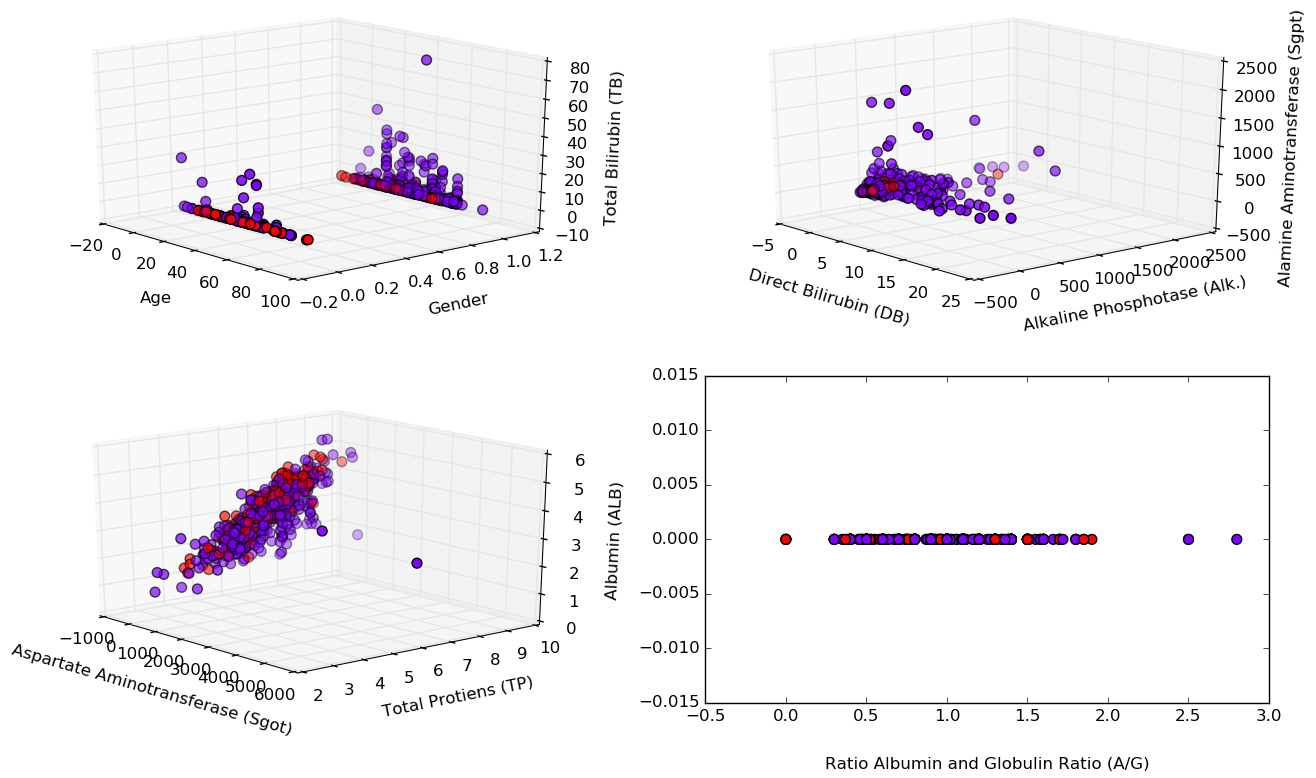
\includegraphics[scale=.4]{experiments/displaying_ilpd}
	\caption{The data set ILPD's samples mapped onto the $\mathbb{R}^n$, where each of its features is an axis in one graph, except for $S \coloneqq \{1, 2\}$, which was represented by the vertices' colors.}
	\label{fig:disp_ilpd}
\end{figure}

As many graphs required to display the data set, it is quite difficult to identify a plausible distribution for ILPD. We define here our first encouragement towards the study of dimensionality reduction: the identification of the most significant features (i.e., that maximize variance) and plotting of those might result on simpler and more intuitive representations. Furthermore, it would also be interesting to combine the existing features to create new ones that are even more representative.

\subsection{Modern Problems and Applications}

Differently from Iris flower or ILPD data set, data sets associated with modern problems are often very dense, i.e., data sets containing many samples and/or features. Although the high number of samples is essentially benefic, a high number of features might be irrelevant or even unconstructive to the learning process \cite{cay2005}. The Leukemia data set, illustrated in the table \ref{tb:ds_leukemia}, is an example of extremelly high dimensionality data set, as it is a sub set of the $\mathbb{R}^{7130}$.

\begin{table}[H]
	\centering
	\begin{tabular}{ c | *{5}{|c}| }
		& F1 & F2 & … & F7129 & F7130 \\ \hline
		1 & -1.46236  & -0.645135 & ... & -0.959575 & 1 \\
		2 & -0.664799  & 0.206146 & ... & -0.543433 & 1\\
		3 & -0.200487  & 0.379941 & ... & -0.896774 & 1\\
		… & … & … & … & … & ... \\
		72 & -0.455835 & -0.071517 & ... & -0.068667 & 1\\
	\end{tabular}
	\caption{The Leukemia data set, with 72 samples and 7130 features \cite{lichman2013}.}
	\label{tb:ds_leukemia}
\end{table}

In many cases, there are indicatives that the data set lie near a lower-dimensional manifold embedded in the $\mathbb{R}^n$ \cite{gho2006}; that is, there is a smaller set of features which roughly express the information within. A second encouragement can then be set: it is possible that the data set might be shrunk by combining similar (linearly dependent) features or eliminating the ones that poorly contribute towards the learning process. In order to do this, one must be able to qualify the “contribution” of each feature or even identify dependencies between features.

\section{Probability Theory}
\subsection{Feature Normalization and Standardization}
Many of the methods ahead will require the data set to be centered in the origin. This is equivalent to remove the mean from each one of the data set's features.

Let $[\vect X]_{n \times f}$ be a data set, $\vect X_{.j}$ the $j$-th column of the matrix $\vect X$, $\mu_j$ the mean of $\vect X_{.j}$ and $\vect 1_n$ the column vector of 1's, we build a \textbf{normalized} data set $\vect X'$ s.t. each column has zero mean:
$$\vect X'_{.j} = \vect X_{.j} - \mu_j \vect 1_n$$

If $\sigma_j$ is the standard deviation of $X_{.j}$, it is also possible to build the \textbf{standardized} $X'$, where each column has zero mean and it is contracted by its standard deviation:
$$X'_{.j} = \frac{X_{.j} - \mu_j \vect 1_n}{\sigma_j}$$

\subsection{Centering Matrix}
The symmetric matrix $\vect H$ is named the \textbf{centering matrix} when the multiplication of it by a matrix $\vect X$ produces the same effect of subtracting the mean of the components from each component of $\vect X$. $\vect H$ is defined as:
$$
\vect H = \vect I_n - \frac{1}{n}\vect{11}^\top \textnormal{, where:}
$$
\begin{enumerate}
	\item $\vect I_n$ is the identity matrix of order $n$.
	\item $\vect 1$ is the column vector of 1's.
\end{enumerate}

\subsection{Variance}
Variance is the measure which describes how far the samples in a given set $X$ vary. For the scope of this project, only discrete probabilities will be considered. That is, if $X$ represents a random variable with known distribution $P(x)$, where $P(x) = k \in \mathbb{R}^{+}, \forall x \in X$ and $\sum_{x \in X} P(x) = 1$, $\mu$ is the population mean of $X$ and $\vect 1_n$ is the column vector of 1's, then, for $n$ samples of $X$ \cite{ross2010introductory}:
\begin{align*}
	Var(X) = \frac{1}{n} (X-\mu \vect 1_n) \cdot (X-\mu \vect 1_n) = \frac{1}{n} \sum_{x \in X} (x - \mu)^2
\end{align*}

\begin{example}
	If $X=\{1, 2, -2, 4\}$ and $\mu = \frac{1}{n} \sum_{x \in X} x = \frac{1+2-2+4}{4} = 1.25$, then
	\begin{align*}
	var(X) &= \frac{1}{n} \sum_{x \in X} (x - \mu)^2 \\
	&= \frac{(1-1.25)^2 + (2-1.25)^2 + (-2-1.25)^2 + (4-1.25)^2}{4} \\
	&= 4.6875
	\end{align*}
\end{example}

\begin{example}
	The variance of the Sepal length feature $\vect X_{.0}$ in the Iris flower data set can be calculated as:
	\begin{align*}
	var(X) &= \frac{1}{150} \sum_i (x_{i,0} - \mu)^2 \\
	&= \frac{1}{150} [(5.1-5.84)^2 + (4.9-5.84)^2 + \cdots + (5.9-5.84)^2] \\
	&= \frac{102.17}{150} = .681122
	\end{align*}
\end{example}

Let $[\vect X]_{n \times f}$ be a data set, $\mu_j$ the mean of the $j$-th column of $\vect X$ and $\vect 1_n$ the column vector of 1's. If $var(\vect X_{.j}) = 0, \forall j \in [0, f)$, then all samples in $\vect X$ are the same.
\begin{proof}
	\begin{align*}
	Var(\vect X_{.j}) &= 0 \\
	\frac{1}{n} (\vect X_{.j} - \mu_j \vect 1_n) \cdot (\vect X_{.j} - \mu_j \vect 1_n) &= 0 \\
	\vect X_{.j} - \mu_j \vect 1_n &= 0  \\
	\iff& \\
	\vect X_{.j} &= \mu_j \vect 1_n
	\end{align*}
	
	All elements in $\mu_j \vect 1_n$ are the same. Therefore $\vect X_{ij} = \mu_j, \forall i \in [0, n)$.
\end{proof}

\subsection{Covariance}

The covariance measures the variance of two random variables in respect to each other. Formally, if $X$ and $Y$ are two given random variables with known mean population distribution $\mu_X$ and $\mu_Y$, respectively, then
$$\sigma(X, Y) = \frac{1}{n} (X - \mu_X) \cdot (Y - \mu_Y) $$

Simply putting, the covariance of two random variables $X$ and $Y$ can be interpreted as one of the following behaviors:
\begin{itemize}
	\item $\sigma(X,Y) > 0$ X tends to increase as Y increases.
	\item $\sigma(X,Y) < 0$ X tends to increase as Y decreases.
	\item $\sigma(X,Y) = 0$ X and Y are completely unrelated.
\end{itemize}

\begin{remark}
	For a random variable $X$, $Var(X) = \sigma(X, X)$.
\end{remark}

\paragraph{Covariance Matrix of Features in a Centered Data Set}

Let $\vect X$ be a data set, $\vect X'$ the data set $\vect X$ with its features centered ($\vect X'=\vect H \vect X$), and $\vect X'_{.j}$ the {\em j-th} feature column of the centered data set $\vect X'$, the covariance between each pair of features can be represented by the matrix:
\begin{align*}
\vect \Sigma_X &= [\vect \sigma_{xy}]_{n \times n} \\
&= \begin{bmatrix}
\sigma(\vect X'_{.0}, \vect X'_{.0}) & \sigma(\vect X'_{.0}, \vect X'_{.1}) & \cdots & \sigma(\vect X'_{.0}, \vect X'_{.n-1}) \\
\sigma(\vect X'_{.1}, \vect X'_{.0}) & \sigma(\vect X'_{.1}, \vect X'_{.1}) & & \sigma(\vect X'_{.1}, \vect X'_{.n-1}) \\
\vdots &&& \vdots \\
\sigma(\vect X'_{.n-1}, \vect X'_{.0}) & \sigma(\vect X'_{.n-1}, \vect X'_{.1}) & \cdots & \sigma(\vect X'_{.n-1}, \vect D_{.n-1})
\end{bmatrix} \\
&= \frac{1}{n} (\vect X')^\top \vect X' \\
&= \frac{1}{n} (\vect{HX})^\top \vect{HX} \\
&= \frac{1}{n} \vect X^\top \vect H^\top \vect{HX} \\
 &= \frac{1}{n} \vect X^\top \vect{HX}
\end{align*}

\section{Numerical Analysis}
\subsection{Eigenvalues and Eigenvectors of a Matrix}

Given a matrix $\vect A \ne 0 \in \mathbb{R}^{2n}$, a vector $\vect v \in \mathbb{R}^n$ is said to be an \textbf{eigenvector} of $\vect A$ if the multiplication $\vect{Av}$ does not change the direction of $\vect v$; that is:
$$\exists \lambda \in \mathbb{R} \mid \vect{Av} = \lambda \vect v \textnormal{, where}$$
$\lambda$ is the \textbf{eigenvalue} associated to the eigenvector $\vect v$.

\subsection{Spectral Decomposition of a Matrix}

If $[\vect A]_{n\times n}$ is a symmetric matrix of rank $n$ and admits $n$ pairs of eigenvalues $\vect \lambda = diag(\lambda_0, \lambda_1, ... \lambda_{n-1})$ and eigenvectors $[\vect V]_{n\times n} = [\vect v_0, \vect v_1, \vect v_2, ..., \vect v_{n-1}]$, such that $\vect V$ is an orthogonal matrix (i.e., $\vect V^\top \vect V=\vect I_n$), then
$$\vect{AV} = \vect{V \lambda}$$

$\vect \lambda$ is a diagonal matrix, where $\lambda_{ii}$ is the eigenvalue associated to the eigenvector $\vect v_i$ \cite{cox2001}. Furthermore, the columns of $\vect V$ are linear independent, hence $\vect V$ is invertible.
\begin{align*}
	\vect{AV} &= \vect{V \lambda} \\
	\vect{AVV^\top} &= \vect{V \lambda V^\top} \\
	\vect A &= \vect{V \lambda V^\top}
\end{align*}

\subsection{Singular Value Decomposition}
\label{sec:svd}
Let $[\vect A]_{n\times n}$ be a matrix, then $\exists \vect U \in \mathbb{R}^{m \times m}, \vect V \in \mathbb{R}^{n \times n}$ and $\vect \Sigma =  diag(\sigma_0, \dots, \sigma_{n-1})$ conditioned to $\sigma_i \ge \sigma_{i+1} \ge 0, \forall \sigma \in [0, n)$ s.t. \cite{gan2008}
$$\vect M = \vect{U\Sigma V^\top}$$

\subsubsection{Decomposition of Symmetric Matrices}
	\label{th:svd-aat}
	If $\vect A = \vect {U \Sigma V^\top}$, $\vect{AA^\top} = \vect{U \Sigma^2 U}$ and $\vect{A^\top A} = \vect{V \Sigma^2 V}$.
\begin{proof}
	\begin{align*}
	\vect{A^\top A} &= (\vect{U\Sigma V^\top})^\top (\vect{U\Sigma V^\top}) \\
	&= \vect{V \Sigma^\top U^\top U \Sigma V^\top} \\
	&= \vect{V \Sigma \Sigma V^\top} \\
	&= \vect{V \Sigma^2 V^\top}
	\end{align*}
\end{proof}

Proving $\vect{AA^\top} = \vect{U \Sigma^2 U^\top}$ is analogous to the above.

\section{Topology}
\subsection{Manifolds}

Intuitively, $n$-dimensional topological manifolds are sets that are ``locally Euclidean" \cite{lee2009}. In other words, they can be decomposed into sub sets that can be mapped to the $\mathbb{R}^n$.

Formally, a set $M$ is said to be a \textbf{$n$-dimensional topological manifold} $\iff M$ is a paracompact Hausdorff topological space $\mid \forall p \in M, p \in U_p$, where $U_p$ is an open set that is homeomorphic to an open set $V_p$ of the Euclidean space $\mathbb{R}^n$ \cite{lee2009}.

\begin{figure}[H]
	\centering
	\captionsetup{justification=centering}
	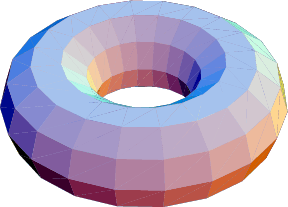
\includegraphics[scale=.4]{manifold/torus}
	\caption{The Torus, often studied in topology, it is a manifold that can be mapped to the $\mathbb{R}^2$ \protect\footnotemark.}
	\label{fig:mani_torus}
\end{figure}

\footnotetext{From ``Torus," by E. W. Weisstein, \textit{MathWorld--A Wolfram Web Resource}. Available at: \href{http://mathworld.wolfram.com/Torus.html}{mathworld.wolfram.com/Torus.html}.}

From now on in this report, we will use the word manifold to refer to a $n$-dimensional topological manifold.

\subsubsection{Charts}
The pair $(U_i, \phi_i)$ is called a \textbf{coordinate chart} or \textbf{chart} on $M$ if $U \in M$ and $\phi_i$ is a \textbf{homeomorphism} such that $\phi_i(U_i) = V_i \subseteq \mathbb{R}^n$ \cite{lee2002}.

\begin{figure}[H]
	\centering
	\captionsetup{justification=centering}
	
	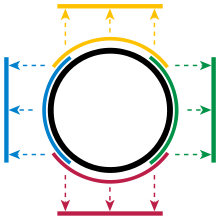
\includegraphics[scale=.4]{manifold/charts}
	\caption{Charts mapping four regions of a circle to different open sets \protect\footnotemark.}
	\label{fig:mani_charts}
\end{figure}

\footnotetext{From ``Manifold," \textit{Wikipedia - The Free Encyclopedia}. Available at: \href{https://en.wikipedia.org/wiki/Manifold}{wikipedia.org/wiki/Manifold}.}

\subsubsection{Atlas}
A set $A = \{(U_i, \phi_i)\}_{i \in A}$ is said to be an \textbf{atlas} on a manifold $M$ if $\cup_{i \in A} U_i = M$ \cite{lee2002}.

\begin{example}
	The $\mathbb{R}^n$ is, directly, a manifold.
\end{example}

\begin{example}
	A n-dimensional sphere is a manifold. Earth, in special, is a 3-dimensional sphere and its stereographic projection (figure \ref{fig:stereographic_earth}) is its mapping to the $\mathbb{R}^2$ \cite{stereo_proj}.

	\begin{figure}[H]
		\centering
		\captionsetup{justification=centering}

		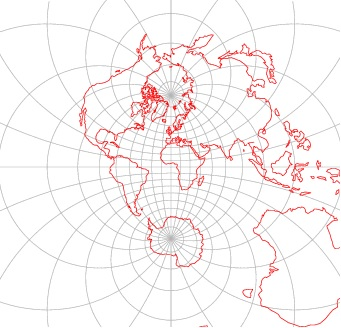
\includegraphics[scale=.8]{manifold/stereo_earth}
		\caption{Stereographic projection applied to Earth \cite{stereo_proj}.}
		\label{fig:stereographic_earth}
	\end{figure}
\end{example}

\subsection{Embedding}

When talking about the relationship between two topological objects, such as two spaces, manifolds or graphs (section \ref{sec:graphs}); it is interesting to imagine a mapping from one object to the other that somehow preserves its original properties.

Let $A$ and $B$ be two topological objects of the same type, a function $\phi \colon A \to B$ is an embedding of A into B if $\phi$ is an isomorphism which preserves the original properties of A \cite{burris2011course}, where such properties are relative to the type of the objects at hand. Shortly, A is said to be \textit{embedded} in B.

\begin{example}[Embedding of Spaces]
	Consider the vector spaces $\mathbb{R}^p$ and $\mathbb{R}^q, p \leq q, p > 0$ and the isomorphism $t \colon \mathbb{R}^q \to \mathbb{R}^t \mid t(x) = [x | \bar{0}] = y$, where $y$ is the vector $x$ concatenated with $p-q$ zeros. $\mathbb{R}^p$ is embedded on $\mathbb{R}^q$, as the operations sum and scalar multiplication are preserved.
\end{example}

\begin{example}[Embedding of Manifolds]
	Let A and B be two manifolds. A is embedded in B if the open sets in A are preserved in B.
\end{example}


\section{Graph Theory}
\label{sec:graphs}
\subsection{Graphs}

Let $G$ be the pair $(V, E)$. $G$ is defined as a \textbf{graph} \cite{berge1973}, where
\begin{enumerate}
	\item $V$ is a set of objects called \textbf{vertices}.
	\item $E$ is a family of elements $e_i \in V\times V$ called arcs.
\end{enumerate}

\begin{figure}[H]
	\centering
	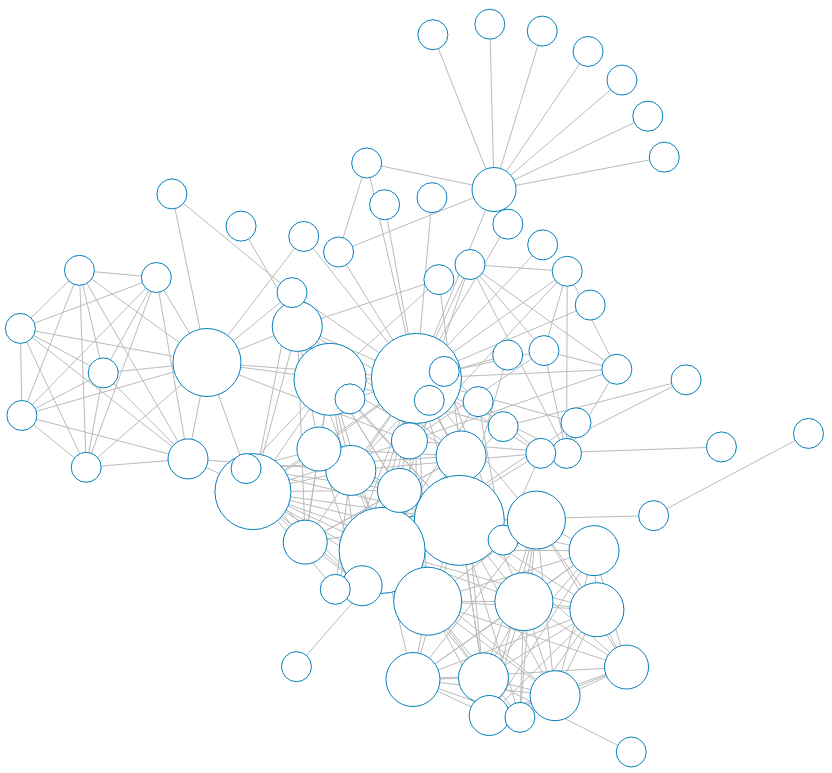
\includegraphics[width=.4\linewidth]{graphs/graph}
	\caption{An example of a graph \protect\footnotemark.}
\end{figure}

\footnotetext{From ``OR-Notes," by J. E. Beasley. Available at: \href{http://people.brunel.ac.uk/~mastjjb/jeb/or/graph.html}{brunel.ac.uk/~mastjjb/jeb/or/graph.html}.}

\subsubsection{Basic Concepts \cite{berge1973}}
\begin{description}
	\item[Multiplicity] If $G=(V, E)$ and $(x, y) \in E \subset V\times V$, the multiplicity $m_g^+(x, y)$ is defined to be the number of arcs with initial endpoint $x$ and terminal endpoint $y$. Furthermore:
	\begin{enumerate}
		\item $m_G^-(x, y) = m_G^+(y, x)$
		\item $m_G(x, y) = m_G^+(x, y) + m_G^-(x, y)$
	\end{enumerate}

	\item[Degree] If $G=(V, E)$ is a graph and $v\in V$, the degree $d(v)$ of $v$ is defined as
	$d(v) = 2n_s  + n_n$, where $n_s$ is the number of arcs self-incident at $v$ \cite{may1972} (i.e., arc with $v$ as initial endpoint and terminal endpoint) and $n_n$ is the number of arcs incident at $v$.

	\item[Adjacency Matrix] If $V=\{v_1, v_2, \dots, v_n \}$ and $G=(V, E)$, define the adjacency matrix $\vect A=[a_{ij}]_{n\times n}$ associated with graph $G$, where $a_{ij} = m_G^+(v_i, v_j)$.
\end{description}

\subsubsection{Further Specifications}

\begin{description}
	\item[Undirected graph] Let $G=(V, E)$ be a graph and $e_k \in E \mid e_k=(a, b) \in E$. The element $e_i=[a, b]$ can be defined as the \textbf{edge} that links $a$ to $b$ without specifying direction. Finally, define the \textbf{undirected graph} $G'$ as $(V, E')$, where $E'=\{e_i\}$ is the set of edges created from $E$ \cite{berge1973}.

	Figure \ref{fig:graph} shows the graph \textbf{Les Miserables}, where each vertex is a character and each arc links two characters that have shared stage at some point during the play. The size of each vertex is a result of its own multiplicity.

	\begin{figure}[H]
		\centering
		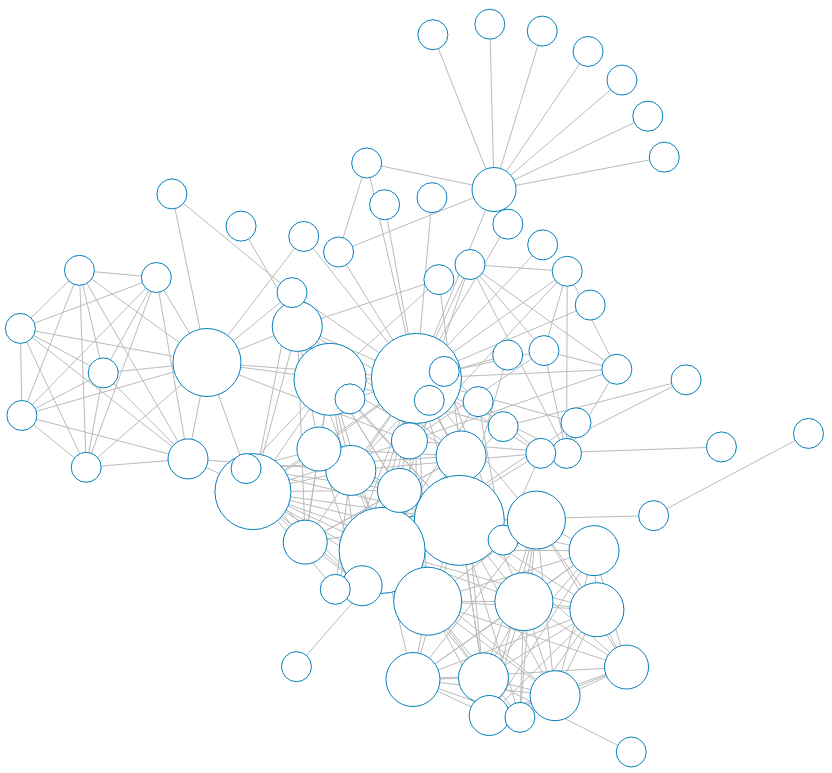
\includegraphics[width=.5\linewidth]{graphs/lesmiserables}
		\caption{The \textbf{Les Miserables} graph \protect\footnotemark.}
		\label{fig:graph}
	\end{figure}
	
	\footnotetext{From ``Graph Theory," by L. David, 2012. Available at: \href{https://comp-ufscar.github.io/graph-theory}{comp-ufscar.github.io/graph-theory}.}
	
	\item[Complete graph] A graph $G=(V, E)$ is said to be complete if
	$$\forall (x, y)\in E, x\ne y, m_G(x, y) \ge 1$$

	\begin{remark}
		Let $G=(V, E)$. $G$ is called the complete graph $K_n$ if $E = V \times V$. That is,
		$$\forall (x, y)\in V \times V, \exists e \in E \mid e=(x, y)$$
	\end{remark}

	\item[Weighted graph] Let $G=(V, E)$ be a graph and $w\colon E \to \mathbb{R} \mid w(e) = w_e$ be the weight associated with arc $e$. $G$ is said to be a weighted graph.

	\item[Euclidean graph] If $G=(V, E)$ and $W=\{w_e, \forall e\in E\}\subset \mathbb{R}$, $G$ is said to be an Euclidean graph if $w_e$ corresponds to the euclidean distance between the vertices connected by $e$ in a given vector space.

	\item[Tree] Let $G$ be the graph $(V, E)$ such that $G$ is connected and admits no cycles. $G$ is  said to be a \textbf{tree} \cite{berge1973}. 

	\begin{figure}[H]
		\centering
		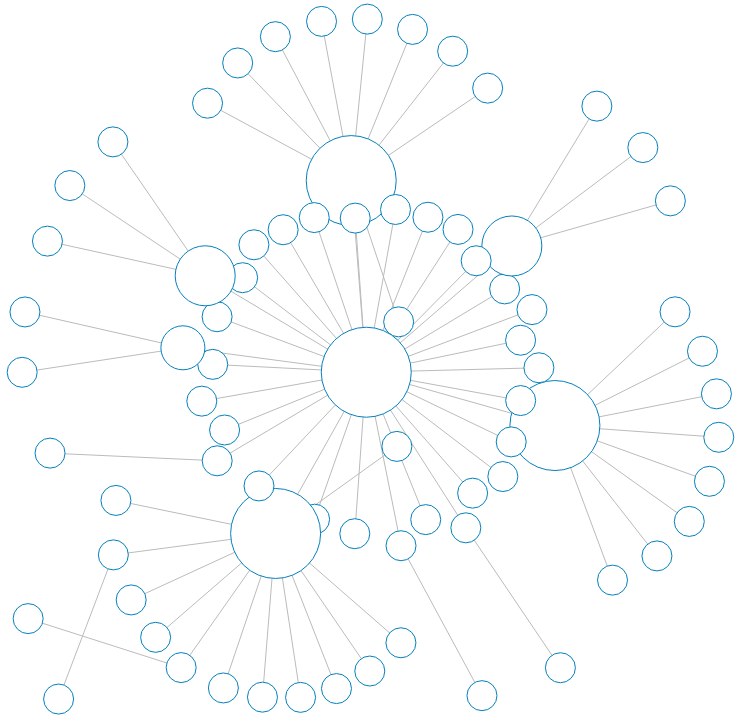
\includegraphics[width=.5\linewidth]{graphs/tree}
		\captionsetup{justification=centering}
		\caption{A tree extracted (a subgraph) from the \textbf{Les Miserables} graph \protect\footnotemark.}
		\label{tree}
	\end{figure}
	
	\footnotetext{From ``Graph Theory," by L. David, 2012. Available at: \href{https://comp-ufscar.github.io/graph-theory}{comp-ufscar.github.io/graph-theory}.}
\end{description}

\clearpage
\subsection{Related Problems}

\subsubsection{Nearest-Neighbor Search}

Let $G = (V, E)$ be a weighted graph, where $w \colon E \to \mathbb{R}$ is the weight or \textbf{length} of the arc $e$, and $n\colon E \to \{0, 1\}$ is a definition of \textbf{nearness} in $G$. The nearest-neighbor search is a optimization problem that consists of finding a subgraph $G' = (V, F \subseteq E) \mid f \in F \iff n(f) = 1$. In other words, to find a subgraph where each arc connects two vertices if and only if these vertices are ``close".

\paragraph{$K$-Nearest-Neighbor Search ($K$-NN)}
Consider $k \in \mathbb{N}$. $K$-NN will result in a subgraph $G'$ s.t. each vertex $v$ is connected at most to $k$ other vertices and the sum of weights of the arcs incident on $v$ is minimum:

\begin{listing}[H]
\begin{minted}[linenos,bgcolor=bgCode]{python}
def nearest_neighbors(V, E, w, k):
    neighbors = set()
    for v in V:
        vs = V - {v}
        # Sort vertices by their how close they are to v.
        vs = sort(vs, keys=[w((v, u)) for u in vs])
        # Keep only k-first vertices.
        vs = vs[0:k]
        neighbors.add(vs)
    return V, neighbors
\end{minted}
\caption{$K$-Nearest Neighbors Algorithm.}
\end{listing}

\paragraph{$\epsilon$-Nearest Neighbor Search ($\epsilon$-NN)}
	Fixed $\epsilon \in\mathbb{R}$, $\epsilon$-NN will find the subgraph $G'=(V, E')$ s.t. each arc in $E'$ has associated weight $w(e) \leq \epsilon$:
	
\begin{listing}[H]
\begin{minted}[linenos,bgcolor=bgCode]{python}
def nearest_neighbors(V, E, w, epsilon):
    neighbors = set()
    for v in V:
        vs = {u for u in V - {v} if w(v, u) > epsilon}
        neighbors.add(vs)
    return V, neighbors
\end{minted}
\caption{$\epsilon$-Nearest Neighbors Search Algorithm.}
\end{listing}

\begin{example}
	If $k=1$ and $\epsilon=60$, the graph $G$, the sub-graph $G'$ found from K-Nearest neighbor algorithm and the sub-graph $G''$ found from the $\epsilon$-Nearest neighbor are defined as follows:
	\begin{figure}[H]
		\begin{subfigure}{.33\linewidth}
			\centering
			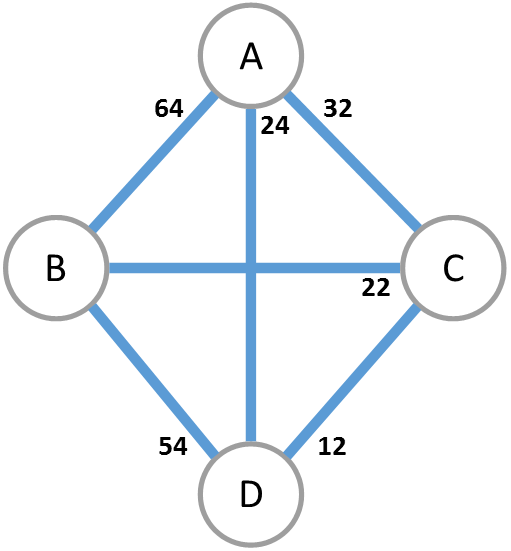
\includegraphics[width=.8\linewidth]{graphs/example-graph}
			\caption{$G$}
			\label{fig:example-graph}
		\end{subfigure}%
		\begin{subfigure}{.33\linewidth}
			\centering
			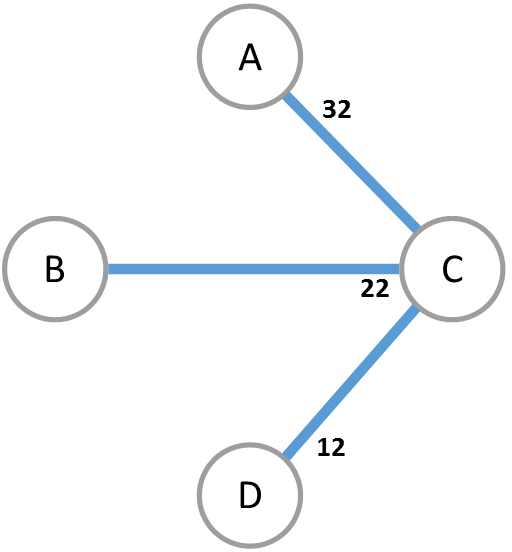
\includegraphics[width=.8\linewidth]{graphs/example-graph-nn}
			\caption{$G'$}
			\label{fig:example-graph-nn}
		\end{subfigure}%
		\begin{subfigure}{.33\linewidth}
			\centering
			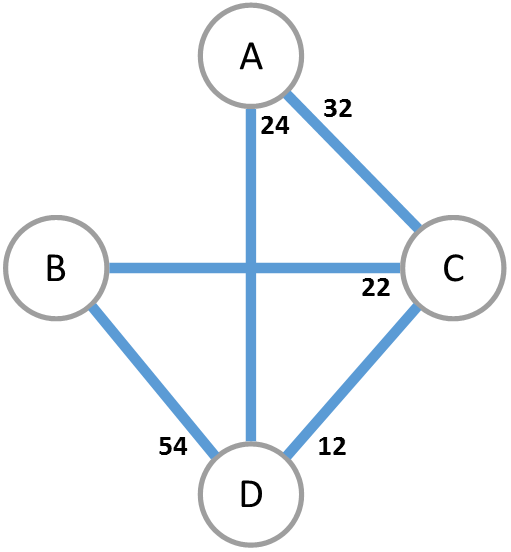
\includegraphics[width=.8\linewidth]{graphs/example-graph-en}
			\caption{$G''$}
			\label{fig:example-graph-en}
		\end{subfigure}
		\caption{The original graph $G$ and the results of $K$-NN and $\epsilon$-NN, respectively.}
	\end{figure}
\end{example}

\clearpage
\subsubsection{Single-pair Shortest-path Problem \cite{cor2011}}

Let $G=(V, E)$ be a weighted graph, $w \colon E \to \mathbb{R}$ and $w(e)$ the weight associated with the arc $e$. Furthermore, consider the paths in $P_{x \to y}=\{(x, v_1, v_2, \dots, y) \mid v_i \in V, \forall i \in (0, n)\}$ and their weights, defined as $w(p) = \sum_0^{n-1} w(p_i, p_{i+1})$.

Under the conditions above, a path $p \in P$ is said the \textbf{shortest-path} between $x$ and $y \iff w(p) \leq w(q), \forall q \in P$. Additionally, the shortest-path weight between two vertices $x$ and $y$ is defined as:
\begin{align*}
	\sigma(x, y) = \begin{cases}
		\min \{w(p(x, y))\}, \text{ if $p(x, y)$ exists}, \\
		\infty, \text{ otherwise.}
	\end{cases}
\end{align*}

The shortest-path between a vertex $x_0 \in X$ and all other vertices can be expressed by the tree $S=(V, F), F \subseteq E$ named \textbf{shortest-path tree}.

\paragraph{Dijkstra's Algorithm}

Let $G=(V, E)$ be a directed weighted graph and $v_0 \in V$ the initial vertex, the shortest-path from $v_0$ to all other vertices can be found through Dijkstra's algorithm:
\begin{listing}[H]
\begin{minted}[linenos,bgcolor=bgCode]{python}
def dijkstra(V, E, w):
    predecessor = {v: None for v in V}
    d = {v: infinity for v in V}
    S = {}
    Q = priority_queue(V, d)
	
    while len(Q) > 0:
        u = Q.pop_min()
        for v in V:
            if d[v] > d[u] + w(u, v):
                d[v] = d[u] + w(u, v)
                predecessor[v] = u
    return (predecessor, d)
\end{minted}
\caption{Dijkstra's algorithm \cite{cor2011}.}
\end{listing}


\begin{remark}
	Dijkstra's algorithm is based on two strategies: greedy, when extracting the vertex $u$ such that $d(u)$ is minimum, and dynamic programming, during edge relaxation (comparison and update of the $d(v)$ and $predecessor(v)$ values).
\end{remark}

\begin{example}
	Let G be the weighted graph as defined in figure \ref{fig:spa-graph}. The shortest-path between $A$ and all other vertices is described by the tree $S$ illustrated in figure \ref{fig:spa-tree}.

	\begin{figure}[H]
		\centering
		\begin{subfigure}{.4\linewidth}
			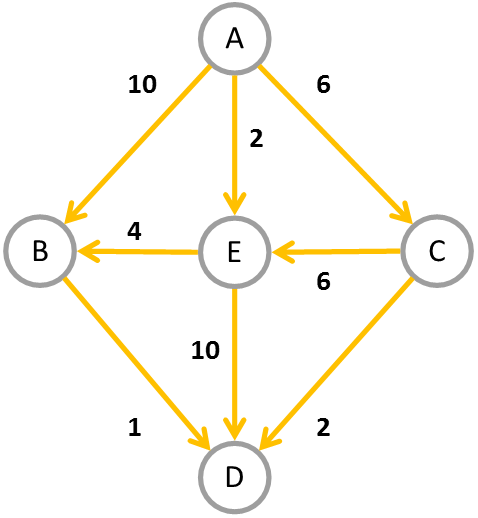
\includegraphics[width=\linewidth]{graphs/spa-graph}
			\captionsetup{justification=centering}
			\caption{The weighted graph $G$.}
			\label{fig:spa-graph}
		\end{subfigure}
		\begin{subfigure}{.4\linewidth}
			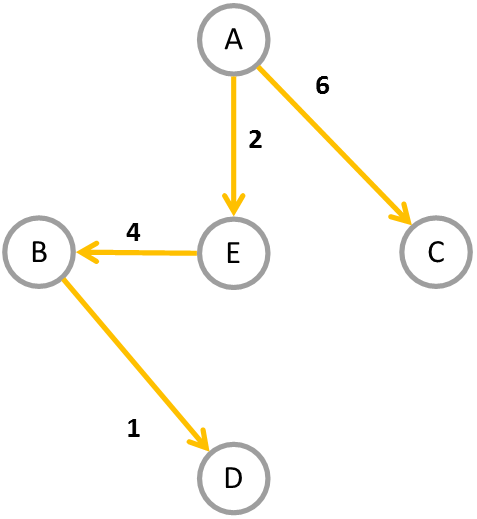
\includegraphics[width=\linewidth]{graphs/spa-tree}
			\captionsetup{justification=centering}
			\caption{The shortest-path tree $S$.}
			\label{fig:spa-tree}
		\end{subfigure}
	\end{figure}
\end{example}

\subsubsection{All-pairs Shortest-path Problem}

Similarly from the previous problem, all-pairs shortest-path is also a search problem that aims to find the predecessors of each vertex $v_i \in V$. The difference is that there is no constraint regarding the initial vertex, i.e., one is interested in finding the shortest routes from every vertex to every other vertex in the graph.

Clearly, all-pairs shortest-path can be solved by executing the Dijkstra's Algorithm $|V|$ times, using every $v_i \in V$ as initial vertex.

\paragraph{Floyd-Warshall Algorithm}

Another solution for the all-pairs shortest-path problem is Floyd-Warshall algorithm, which is entirely based on dynamic programming:

\begin{listing}[H]
\begin{minted}[linenos,bgcolor=bgCode]{python}
def floyd_warshall(V, E, w):
    d = {}
    for v in V:
        for u in V - {v}:
            d[v, u] = w[v, u]

        predecessor[v, u] = None

    for k in V:
        for v in V:
            for u in V:
                if d[u, v] > d[u, k] + d[k, v]:
                    d[u, v] = d[u, k] + d[k, v]
                    predecessor[u, v] = k
      return predecessors, d
\end{minted}
\caption{Floyd-Warshall Algorithm \cite{golin2003floydwarshall}.}
\end{listing}

Now, matrix $d$ contains  the weights sum for the paths between all vertices of the graph. These paths can be constructed by:

\begin{listing}[H]
\begin{minted}[linenos,bgcolor=bgCode]{python}
	def path(i, j, predecessor):
		if predecessor[i, j] == None:
			return [i, j]
		l = path(i, predecessor[i, j])
		r = path(predecessor[i, j], j)
		return l.append(r)
\end{minted}
\caption{Algorithm for path reconstruction from list of predecessors \cite{golin2003floydwarshall}.}
\end{listing}

\clearpage
\section{Machine Learning}
Learning it is Improvement of an agent's performance over a specific environment through acquisition of experience \cite{pat1996}. Machine learning relates to the area in Computer Science which aims to extend the human learning concept to machines. That is, the implementation of machines that can imitate human learning \cite{hot2009}. Practically, this usually translates into creating machines that are able to recognize patterns in an environment and interpret those using concepts related to artificial intelligence. Such interpretation can create a model which might eventually be used to predict new patterns, take actions and/or solve domain problems.

Based on how the learning phase of a problem is, ML algorithms are mostly divided into one of the following categories:

\begin{description}
	\item[Supervised] A direct feedback is presented during the learning phase \cite{pat1996}. For the instances where the ME problem relies on a data set, the learning task uses the labeled training samples (i.e., samples that present the \textbf{target feature}) to synthesize the model that attempts to generalize the relationship between the feature vectors and the target variable \cite{awa2015}.
	
	\item[Unsupervised] Infer hidden structures from the data set without direct feedback, such as known labels for the samples \cite{awa2015}.
	
	\item[Semi-supervised] Most commonly, it is given by the extension of either supervised or unsupervised learning to include the other paradigm, resulting in a combination of both \cite{zhu2009}.
	
	\item[Reinforcement] Through iterative exploration, the learner is positively or negatively reinforced for its actions. The learner's goal is, ultimately, maximize the cumulative reward gained \cite{awa2015}.
\end{description}

Regarding the nature of what is being learned, ML algorithms can be separated between:
\begin{description}
	\item[Classification] Each sample $\vect x$ of the data set $\vect X$ is associated with a label $y_{\vect x} \in \vect Y$, regardless if this label is known or unknown. Moreover $|\vect Y| < \infty$. The ML algorithm goal is to create a model which can infer a label to a given sample.
	\item[Regression] Samples of the data set $\vect X$ follow a regression function $f$. The goal is to learn such function. A reasonable manner to think of it is to imagine the samples of $\vect X$ being associated with continuous labels \cite{kramer2013dimensionality}.
\end{description}

ML algorithms often represent the end-point of the learning process, receiving the result of reduction algorithms as input and learning from them instead of the raw data. In this section, we will study a small set of supervised ML algorithms. Later, we will use them to simulate how the reductions produced by ISOMAP are interpreted by ``real-world" ML algorithms.

\subsection{$K$-Nearest Neighbors}

One might consider using the concepts of locality and proximity to perform classification or regression. $K$-Nearest Neighbors ($K$-NN) can be employed here, being possibly one of the most straight forward methods for prediction \cite{elkan2011nearest}.

\subsubsection{$K$-NN Classifier}

Let $\vect X$ be a data set, $\vect Y$ the array of labels possibly assumed by samples in $\vect X$, $\vect s$ a unlabeled sample and $k \ge 1$ a fixed integer. The $K$-NN classifier will determine $\vect s$'s class based on the most common class shared between $\vect s$'s closest neighbors: if $\vect X_s \subset \vect X$ is the set of neighbors of $\vect s$, consider $E_{\vect X_s}[i]$ the probability of a sample in $\vect X_s$ being associated to the label $i$. Then,
\begin{align*}
	y(\vect s) = \arg \max_{i \in Y} E_{\vect X_s}[i]
\end{align*}

\subsubsection{$K$-NN Regressor}

Let $\vect X$ be a data set, $\vect Y$ the array of instants of the regression function, $\vect s$ a unlabeled sample and $k \ge 1$ a fixed integer.
The $K$-NN regressor attempts to generalize the regression function by averaging the instants in $\vect Y$ associated with $\vect s$'s nearest neighbors \cite{kramer2013dimensionality}, given by $N_k(s)$:	
\begin{align*}
	y(\vect s) = \frac{1}{k} \sum_{\vect x \in N_k(\vect s)} y_{\vect x}
\end{align*}

In order to increase the accuracy in both classification and regression, the importance of the label/instant associated to each neighbor can be weighted by the distance $d$ between it and $\vect s$, where $d$ is defined based on the context of the problem (although the Euclidean distance is broadly employed \cite{elkan2011nearest}).

\subsection{Support Vector Machine}

Contained in the supervised learning category, Support Vector Machine (SVM) is a powerful tool, often used in classification and regression problems.

Intuitively, the SVM classifier attempts to find a hyperplane that separates the samples in a data set into two different groups: positives and negatives (i.e., binary classification). Furthermore, the hyperplane is placed such that the distance between the \textbf{support vectors} (the closest samples) and it are maximized.

\begin{figure}[H]
	\centering
	\captionsetup{justification=centering}

	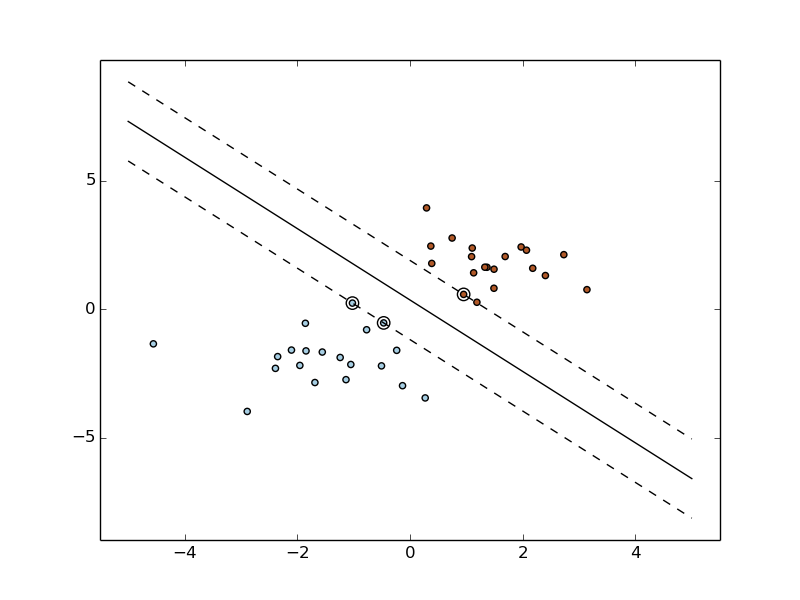
\includegraphics[scale=.5]{ml/svm_margin}
	\caption{A SVM classifier projecting a hyperplane that perfectly separates two classes of samples \cite{sksvm}}.
	\label{fig:svmmargin}
\end{figure}

More elaborately, given any linearly separable data set $\vect X$ containing samples from two distinguished classes $\{-1, +1\}$, consider the vector $\vect w$ and the hyperplane $d = \{\vect x \mid \vect w \cdot \vect x + b = 0\}$ (represented in fig. \ref{fig:svmmargin} by the contiguous line). The class $y_i = y(x_i)$ to which a given sample $\vect x_i$ belongs can be defined as:
\begin{align*}
	y(x_i) = \begin{cases}
		+1, \text{if } \vect w \cdot \vect x_i +b > 0 \\
		-1, \text{otherwise.}
	\end{cases}
\end{align*}

To prevent samples from falling into the margin or being misclassified \cite{wessvmdef}, reinforce that for any positive sample $\vect x_+$, $\vect w \cdot \vect x_+ +b \geq 1$. Similarly for $\vect x_-$ samples, $\vect w \cdot \vect x_- +b \leq 1$. These both constraints can be expressed as
\begin{equation} \label{svmconst}
y_i(\vect w \cdot \vect x_i +b) -1 \geq 0
\end{equation}

Notice that $y_i(\vect w \cdot \vect x_i +b) -1 = 0 \iff \vect x_i $ is a \textbf{support vector}.

The width (the distance between the two margins) of the street is the vector $(\vect x_+^0 - \vect x_-^0)$ projected onto the vector $\vect w$, where $\vect x_+^0$ is a positive support vector and $\vect x_-^0$ is a negative one.
\begin{equation} \label{eq:eqsvmwidth}
\begin{split}
width &= (\vect x_+^0 - \vect x_-^0) \cdot \frac{\vect w}{\|\vect w\|} \\
      &=\frac{\vect x_+^0 \cdot \vect w - \vect x_-^0 \cdot \vect w}{\|\vect w\|} \\
      &=\frac{1-b - (-1-b)}{\|\vect w\|} = \frac{2}{\|\vect w\|}
\end{split}
\end{equation}

As the goal is to maximize the width, while still respecting the constraint (\ref{svmconst}).
\begin{equation} \label{eq:svmminw}
	\max width = \max \frac{2}{\|\vect w\|} \equiv \min \frac{1}{2} \|\vect w\|^2
\end{equation}

Which can be solved using standard quadratic programming.

\subsubsection{SVM for non-separable data sets (soft margins)}

To deal with non-separable data sets, it is possible to introduce the variables $\xi_i$ to the optimizing equation (\ref{eq:svmminw}) and to the decision rule (\ref{svmconst}) \cite{wessvmdef}. This represents a trade-off between maximum margin/distance of the misclassified samples from the decision boundary. The optimizing equation and the decision rule are updated to:
\begin{align*}
	&\min \frac{1}{2} \|\vect w\|^2 + C \sum_{1}^{m}\xi_i \text{, constrained to:} \\
	&y_i(\vect w \cdot \vect x_i +b) \geq 1- \xi_i, \xi_i \geq 0
\end{align*}

Such trade-off can be adjusted through the parameter $C$. Notice that small values for $C$ might result in misclassification, whereas high values can produce overfitting.

\subsubsection{Dependency over the dot product}

Equation \ref{eq:svmminw} does not explicitly illustrates how the model generated depends on the dot product between the training samples. The implications of such fact will be discussed in the next section. For now, let us convert \ref{eq:svmminw} to its dual form. By the Lagrange multipliers method \cite{mitsvm}:
\begin{align} \label{eq:svmlag1}
	L &= \frac{1}{2}\|\vect w\|^2 - \sum \alpha_i[y_i(\vect w \cdot \vect x_i +b) -1] \\
	\label{svmlag2}
	\frac{\partial L}{\partial \vect w} &= \vect w -\sum\alpha_i y_i \vect x_i = 0 \implies \vect w = \sum\alpha_i y_i \vect x_i \\
	\label{svmlag3}
	\frac{\partial L}{\partial b} &= -\sum\alpha_i y_i = 0 \implies \sum\alpha_i y_i = 0
\end{align}

Applying (\ref{svmlag2}) and (\ref{svmlag3}) on (\ref{eq:svmlag1}), our problem of minimizing (\ref{eq:svmminw}) constrained by (\ref{svmconst}) becomes maximizing $L$, subject to (\ref{svmlag3}):
\begin{gather*}
L = \frac{1}{2}\sum\alpha_i y_i \vect x_i \cdot \sum\alpha_j y_j \vect x_j
- \sum \alpha_i y_i \vect x_i \cdot \sum \alpha_j y_j \vect x_j
- \sum \alpha_i y_i b + \sum \alpha_i \\
= \sum\alpha_i -\frac{1}{2}\sum\sum\alpha_i\alpha_j y_i y_j (\vect x_i \cdot \vect x_j)
\end{gather*}

$w$ and $b$ can easily be found from (\ref{svmlag2}) and $\alpha_i[y_i(\vect w \cdot \vect x_i + b) - 1] = 0$ (for any $i \mid \alpha_i \ne 0$), respectively.

Now, as we finally plug (\ref{svmlag2}) back into our decision rule, it becomes clear that both training and prediction phases depend only on the dot product between the sample vectors \cite{mitsvm}:
\begin{align*}
	y(\vect x_k) = \begin{cases}
		+1, \text{if } \sum\alpha_i y_i \vect x_i \cdot \vect x_k +b \geq 0\\
		-1, \text{otherwise.}
	\end{cases}
\end{align*}

\subsubsection{Kernel functions}

"The kernel function represent the dot product of both vectors projected onto the new space". \cite{mitsvm}

Some data sets are not linearly separable, as previously mentioned	. They can, however, be projected to a different vector space, where they hopefully will be. To achieve this, a transformation $\phi$ is applied on both vectors. The dot product between those is then calculated in the new space and the value is used during training and prediction:
\begin{gather*}
L = \sum\alpha_i -\frac{1}{2}\sum\sum\alpha_i\alpha_j y_i y_j \phi(\vect x_i) \cdot \phi(\vect x_j)
\end{gather*}

\begin{remark}
	Practically, Let $k: (\mathbb{R}^n, \mathbb{R}^n) \rightarrow \mathbb{R} \mid k(\vect u, \vect v) = \phi(\vect u) \cdot \phi(\vect v)$, then:
	\begin{align*}
	L &= \sum\alpha_i -\frac{1}{2}\sum\sum\alpha_i\alpha_j y_i y_j k(\vect u, \vect v) \\
	y(\vect x_k) &= \begin{cases}
			+1, \text{if } \sum\alpha_i y_i k(\vect x_i, \vect x_k) +b \geq 0\\
			-1, \text{otherwise.}
		\end{cases}
	\end{align*}
	
	Which entails, given a known function $k$, there is no need to explicitly know which are the projections of $u$ and $v$ onto the new vector space. This is commonly known as the \textbf{kernel trick}.
\end{remark}

The first set of axis $\{x\}$ in the figure bellow illustrates the non-linearly separable distribution of positive and negative samples in the $\mathbb{R}$. The second basis $\{x, y=x^2\}$ represents the same samples being projected to the $\mathbb{R}^2$.

\begin{figure}[H]
	\centering
	\captionsetup{justification=centering}

	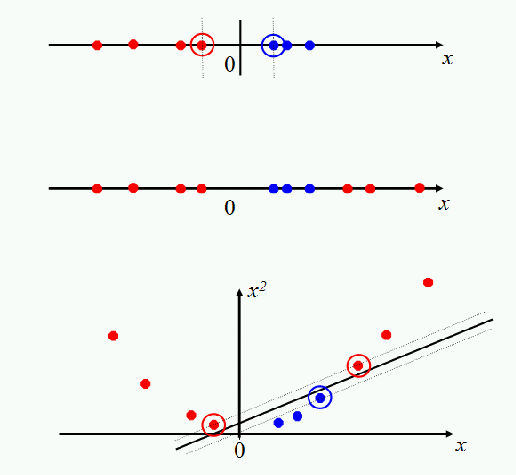
\includegraphics[scale=.4]{ml/svm_kernel}
	\caption{Projection of samples from the $\mathbb{R}$ to the $\mathbb{R}^2$, allowing SVM to find a hyperplane that perfectly separates both classes \cite{svmkernels}.}
	\label{fig:svmkernel}
\end{figure}

Many different kernels exist. Two which are frequently used among all of them\cite{svmkernels} are:
\begin{itemize}
	\item RBF: $\exp(-\frac{\|x -x'\|^2}{2\sigma^2})$
	\item Polynomial: $(u^\top v + c)^{d}$.
\end{itemize}

\subsubsection{Multi-class Classification}

SVMs are constructed over the concept of binary separation, but not all problems are binary. In classification, this reflects data sets that have their samples separated into more than two classes. The Iris flower data set is an example of this, when predicting the samples' {\em species}.

There are many different approaches for multi-class classification \cite{rif2008}. For the scope of this work, consider only the following:

\begin{description}
	\item[One-vs-All (OVA)] $n$ binary classifiers are built, where $n$ is also the number of classes in the data set. For the classifier $c^j, j \in [1, n]$, all samples of the $j$th class are taken as positive samples, at the same time that all the other samples are considered negative.

	If $c^j(\vect x)$, the $j$-th classification of sample $\vect x$, is defined as:
	$$c^j(\vect x) = \sum_{i=1}^{m} \alpha_i^j y_i \vect x \cdot \vect x_i + b$$

	Then positive values for $c^j(\vect x)$ indicate that the sample $\vect x$ belongs to the $j$th class. Additionally, greater $c^j(\vect x)$ values imply on further distance from the hyperplane (i.e., $c^j(\vect x)$ can also be interpreted as a \textbf{confidence value}) and the sample $x$ should be assigned to the class which holds greatest confidence \cite{ovacj}. Shortly, classification is given by
	$$ y(\vect x) = \argmax_j{c^j(\vect x)} $$	
	\item[All-vs-All (AVA)] Also known as all-pairs or one-vs-one, a classifier $c_{ij}$ is built for each pair of classes $(i, j)$, resulting in a total of $n(n-1)$ classifiers. $c_{ij}$ responds with positive values for samples of the $i$-th class and negative values for samples of the $j$-th class. Classification can be done by simply counting the class most frequently associated with $\vect x$:
	$$ y(\vect x) = \argmax_i{\sum_{j=1}^{n} c_{ij}(\vect x)} $$
	Or equivalently, but only using $\frac{n(n-1)}{2}$ classifiers,
	$$ y(\vect x) = \argmax_i{\sum_{j=1}^{n} \frac{j-i}{|j-i|} c_{\min(i, j) \max(i, j)}(\vect x)} $$
\end{description}

\subsection{Evaluating Supervised Learners}

Machine Learning algorithms might be susceptible to data noise, incorrect configuration or even random factors, which would eventually decrease the generated model's accuracy. Additionally, there is also the change of \textbf{overfitting}, the event where a learner performs sufficiently well over the learned data, but fails to make correct predictions over yet-unseen data. In order to evaluate this accuracy, models are quite often tested after trained.

Considering that testing with the same data used for training will most likely produce unreliable results, a simple way to test a learner is to separate the labeled data set into two chunks, where the first is used for training. The second chunk is then be given to the learner, which attempts to predict the samples. Finally, the predictions made by the learner would be compared with the actual labels.

\subsubsection{Confusion Matrix and Prediction Accuracy When Classifying}

To evaluate classification models, one way to visualize the incorrect predictions made by the learner is a \textbf{confusion matrix}, where the item $a_{ij}$ is the number of times that a sample of the class $i$ was classified as being of the class $j$.

\begin{table}[H]
	\centering
	\begin{tabular}{*{4}{c|}c}
          &  a &  b &  c &  d \\\hline
		a & 12 &  3 &  2 &  0 \\
		b &  7 & 12 &  2 &  4 \\
		c &  0 &  4 & 54 &  8 \\
		d &  6 &  0 &  1 & 23
	\end{tabular}

	\caption{Example of confusion matrix for a data-set with four different classes.}
\end{table}

We define the \textbf{prediction accuracy} of a ML model as the number of correct predictions divided by the total number of predictions made:
\begin{align*}
	accuracy = \frac{\sum_i c_{ii}}{\sum_i \sum _j c_{ij}}
\end{align*}

Where $\vect C$ is a confusion matrix.

Naturally, a diagonal matrix $\vect C$ represents that all samples were correctly classified, being the best possible outcome (no errors).

\subsubsection{Prediction Accuracy When Regressing}

The coefficient of determination, which can be interpreted as how much data variance is explained by a prediction model, can easily be used to evaluate regression models.

Let $\vect X$ be a data set, $\vect y_i$ an observation of the regression function associated with the sample $\vect x \in \vect X$, $\vect y_i^p$ the actual value predicted by the regression model and $\bar{\vect y}$ the average of all observations, then:
\begin{align*}
	R^2 = 1 - \frac{\sum_i (y_i^p - y_i)^2}{\sum_i (y_i^p - \bar{\vect y})^2}
\end{align*}

\subsubsection{Cross Validation}

When the estimator at hand accepts different settings (``hyperparameters"), such as $k$ in $K$-NN or $C$ in the SVM, there is still a change of overfitting on the testing set, as these parameters can always be tweaked for optimal performance. In order to avoid this, a third chuck, called validation set, can be divided from the original data set and used to ``validate" the learner current settings.

Sometimes, partitioning the data set into three subsets might be malign to the learning process, as the model will be constructed only considering a small, random portion of the samples (when the data set does not have too many samples, for instance). This event is known as \textbf{underfitting}. Fortunately, cross validation can be used to deal with such cases. When $k$-fold cross-validating \cite{crossvalid}, the data set can be partitioned into $k$ folds. For each fold $k_i$, a model is trained with all folds, except for $k_i$. The model is then tested over $k_i$. Finally, the score reported by the cross-validation method is the average accuracy when testing over all folds.

\subsubsection{Grid Search}

As a learner hyperparameters strongly affect how the generated model will perform, one cannot choose them arbitrarily. Furthermore, when learners have a high number of hyperparameters, it becomes difficult to manually define a ``good" setting for them. For example, SVM requires $C$ and which $kernel$ - and the kernel's own parameters, of course - it should use.

Grid Search is a traditional method used to find the learner's hyperparameters that maximize accuracy optimize the generalization of learning model over a specific data set \cite{gridsearch}. Given a set of possible parameters, it will exhaustively search for the combination of those that generate the best outcome, which might be evaluated by a validation method such as cross-validation.

\subsection{Examples of Learning}

\subsubsection{Coffee Selling Rate}

The figure bellow illustrates the distribution of coffee sales per time of the day in a particular coffee-shop \cite{roh2015}. Clearly being a regression problem, a machine learning algorithm must create a model that appropriately generalizes the distribution observed. Such model will eventually be used to predict the selling rate in the following days.

\begin{figure}[H]
	\centering
	\captionsetup{justification=centering}

	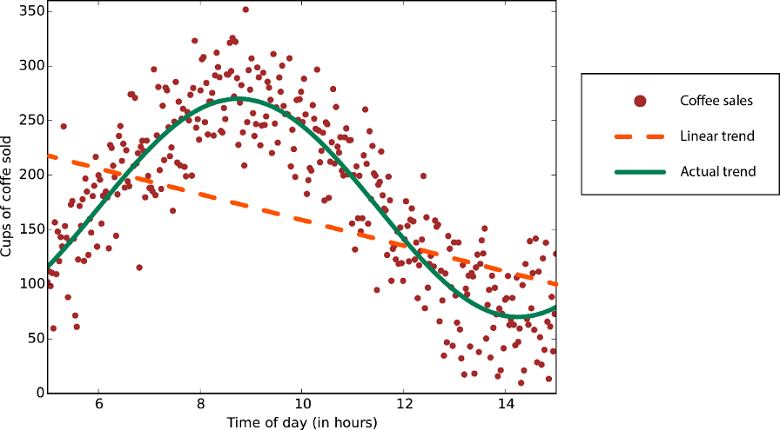
\includegraphics[scale=.4]{ml/rohrer2015}
	\caption{graphic representation of a data set generalization by a linear (orange) and a nonlinear model (green) \cite{roh2015}.}
	\label{fig:rohrer2015}
\end{figure}

The orange line and the green arc represent two different models. The orange line, which represents the linear model, clearly does not generalize the data set appropriately, once it induces an error much larger than necessary \cite{roh2015}. The nonlinear model, i.e., the green arc, was capable of generalize the data inducing a smaller error.

\subsubsection{Iris Flower}

Consider the Iris flower data set as defined in \ref{irisdataset}. In order to predict the feature {\em Species} of a given sample, one could train a Support Vector Machine classifier.

Through GridSearch, it was found that the SVM algorithm with $C=100$, $gamma=.01$ and $rbf$ kernel is capable of finding a model yielding .99\% accuracy. The samples misclassified during the test phase were represented by the confusion matrix bellow.

\begin{figure}[H]
	\centering
	\captionsetup{justification=centering}

	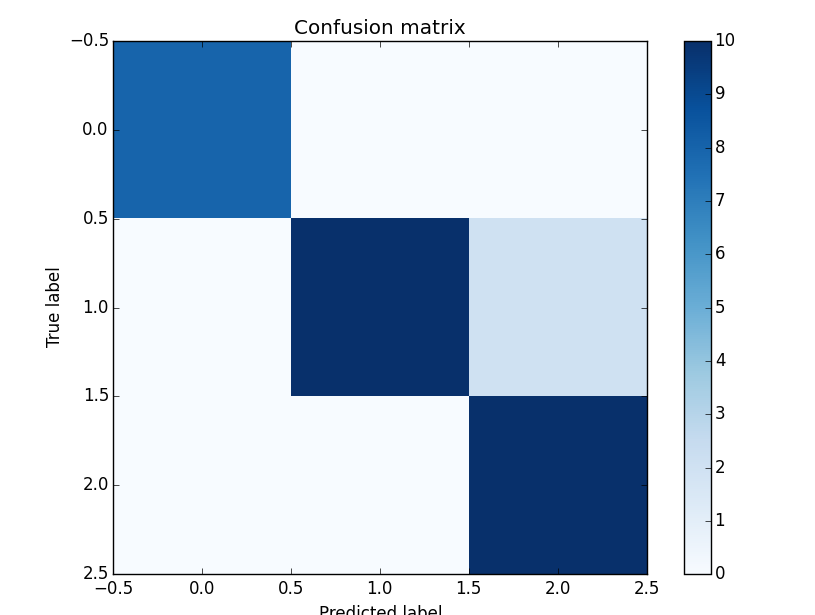
\includegraphics[scale=.2]{ml/svm_cm_iris}
	\caption{Confusion matrix of a SVM with $C=100$, $gamma=.01$ and $rbf$ kernel when predicting samples from the Iris flower data set.}
	\label{fig:cmsvmiris}
\end{figure}
